\section{Results}
\label{sec:results}

\begin{table*}[tb]
  \caption{Objects} \label{tab:objects} \centering
  \begin{tabular}{|c|l|c|c|c|l|}
    \hline
    &Description& Weight(Kg)&No.Trials&No.Failures&Contains \\
    %&Object& W(Kg)&Trials&Fail&Contains \\
    \hline
    0&White Bottle        & 0.265 & 22& 0 & Vitamins\\
    1&White Porcelain cup & 0.255 & 24& 1 & Nothing\\
    2&Startbucks cup      & 0.220 & 24& 4 & Bolts \\
    3&Nesquick box        & 0.240 & 24& 2 & Nesquick powder\\

    \hline
  \end{tabular}
\end{table*}

\begin{figure}[tbp]
\centerline{
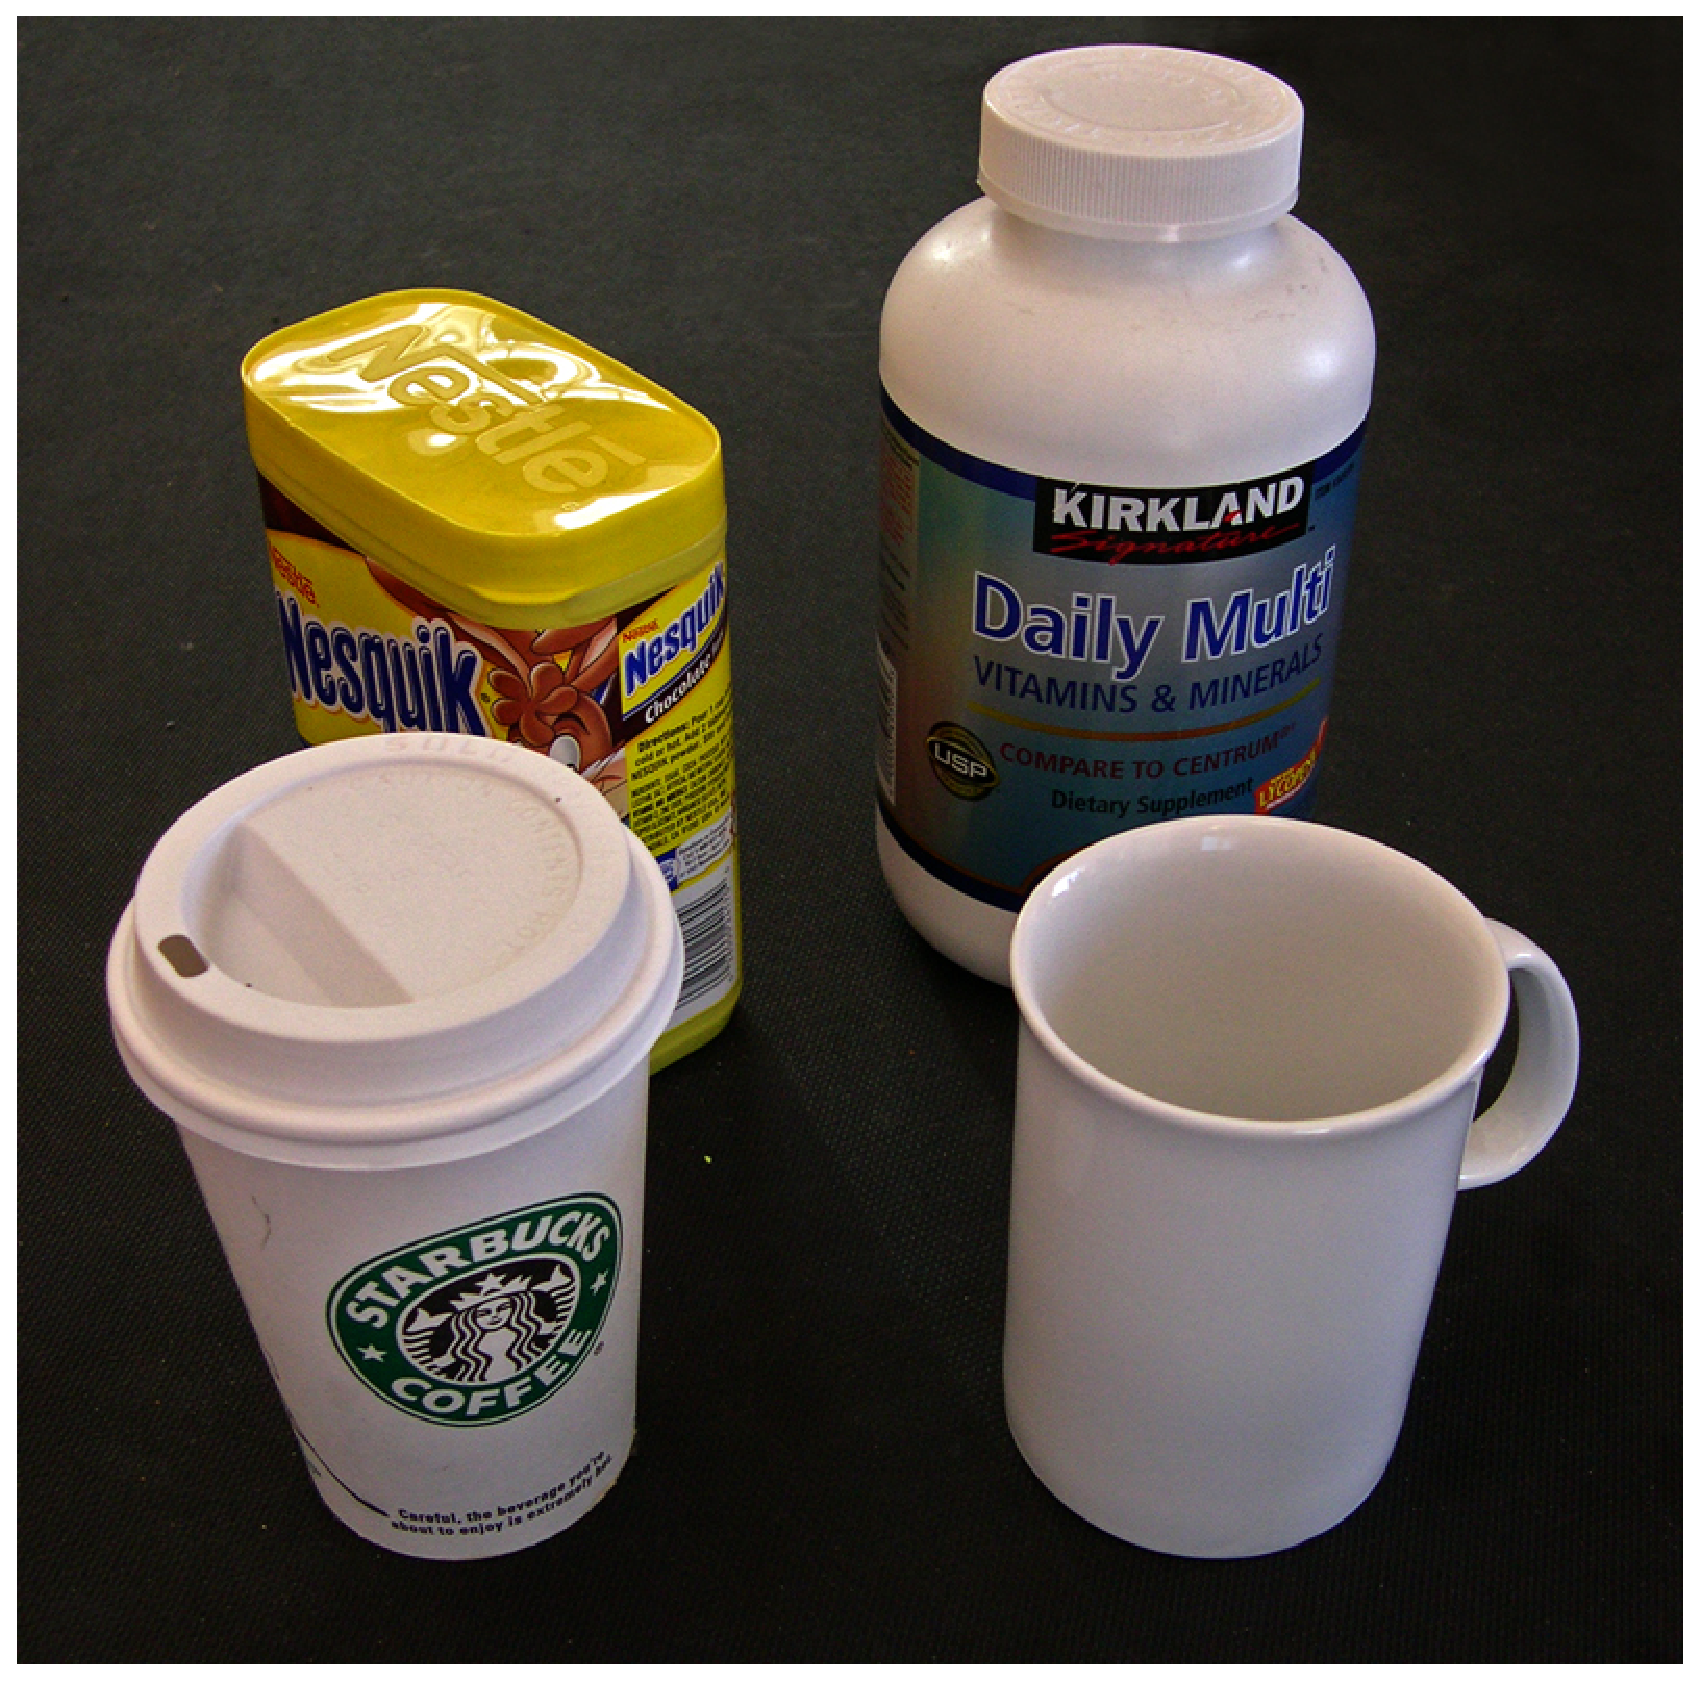
\includegraphics[width=2.0in]{./figures/objects.eps}
}\caption{Objects}
\label{fig:Objects}
\end{figure}

An example resulting from the implementation described in
section~\ref{sec:behavior} is shown in figure~\ref{fig:sequence}.
We can observe the reaching action followed by the positioning and
grasping. [Should we include a plot of the readings of the
sensors?]


Using the behavior described in section~\ref{}, the robot was able
to grab a number of different objects. The robot had no prior
knowledge of the objects. We evaluate the performance by
presenting to the robot many times four objects and counting the
number of times that they were grabbed. Out of 94 trials only 8
failed. The objects were : a white vitamins bottle, a white
porcelain cup, a startbucks cup and a nesquick box. The physical
properties of the objects and the results are shown in table
\ref{tab:objects}.

[No sure if we should include this part]

We have also evaluated the behavior of the tactile sensor grabbing
the same object but with different weights. The object used was
the white bottle and the weights used are presented in the
table~\ref{}.






%We evaluated our work by performing an object recognition
%experiment. We exposed the robot one evening to a set of seven
%objects, and then in the morning tested its ability to recognize
%another set, which had an overlap of four objects with the
%training set. Three of these objects were chosen (Figure 8) to
%represent three different materials, plastic, glass and steel
%(metal). The idea is that the sound produced by each object
%depends on its size, shape and the material with which it is made;
%accordingly we expected the tapping to produce three different
%distinct sounds. A fourth object (a plastic toy) was relatively
%silent. For each run, we placed randomly selected objects on the
%table in front of the robot, and it was responsible for finding
%and tapping them. Overall the robot tapped 53 times; of these
%episodes 39 were successful, meaning that the sound produced by
%the tapping was significantly loud; in the other 14 cases the
%tapping did not provoke useful events either because the initial
%impact caused the object to fall, or the object remained too close
%to the hand. The high number of successful trials shows that given
%the mechanical design of the hand, haptic feedback was sufficient
%to control the interaction between the robot and the environment.
%We evaluated the performance of our spectrum comparison method by
%ranking the strength of matches between episodes on the second day
%and episodes on the first day. Figure 7 shows what detection
%accuracy is possible as the acceptable false positive rate is
%varied. This predicts that we can on average correctly match an
%episode with 50\% of previous episodes involving the same object
%if we are willing to accept 5\% false matches.
